\chapter{Direct backward ray mapping for systems with Fresnel reflection}
\label{chap:fresnel}
% Fresnel's equation give a physically accurate expression for the power transmission and reflection according to angle. For all but some special anhles a ray splits up into a reflected and transmitted ray. Both carry off some of the incident energy. For accurate ray tracing this means that both have to be followed theought optics. However, this splitting happens at each interface
In this chapter we present the backward ray mapping method for systems consisting of optical lines at which Fresnel reflections can occur. In the following we consider unpolarized light and we do not take into account scattering phenomena. In particular, we explain how to calculate the boundaries of the regions of positive luminance in target PS. We provide numerical results for our system formed by the source, a lens and the target. 
The chapter starts with a general introduction of the method, then the details are explained for a simple system, finally we show the results obtained.
\section{Introduction}
Including Fresnel reflections, every time that a ray hits an optical line, it splits into a reflected and a refracted ray, both of them carry a part of the incident energy. In case a ray propagating from a more dense to a less dense medium hits the line with an angle greater than the critical angle, it can be only reflected and TIR occurs (see Section \ref{sec:fresnel}).
%The amount of light that is reflected and refracted is given by the reflectance and transmittance which are related to Fresnel coefficients (see ). 
A part of this case, a ray emitted from the source generates two rays after interaction with the optical line (the reflected ray and the transmitted one) each of them has a fraction of the original power given by the reflectance $\mathcal{R}$ and the transmittance $\mathcal{T}$ obtained from (\ref{Fresnel_pands}).
At the next intersection of the two rays with a line, each incident ray is split
again. This process is called \textit{ray splitting} and results in tracing a rapidly increasing number of rays, including those containing very little power. 
%The ray emitted from the source is called the parent ray. Once it hits a line one of the two rays keeps the parent status while the other one is called child ray. The convention is to assign the parent status to the ray transporting the most power.
Many different paths can occur and the number of paths is determined considering all the possible combinations that a ray emanating from the source can generate. The number of possibilities increases with the number of optical lines that form the system. For example, for a system formed by a source, one single line and a target, two possibilities occur since a ray emitted from the source can either refract reaching the target or reflect going back to the source. If the system is formed by a source, two lines and a target much more paths are possible since the ray can reflect forward and backward between the two optical lines before arriving either at the target or at the source again. For systems where multiple reflections can occur the number of paths can increase dramatically. Ray splitting is a powerful and accurate ray tracing method to calculate \textit{all} physical paths. The disadvantage is that it generates more and more rays, many of which are not significant for computing the target intensity. This makes methods based on ray splitting time consuming. A stopping criterion is needed. Ray generation can be controlled either neglecting rays with a small flux or limiting the total number of interactions that a ray can undergo during its propagation. \\ \indent A different ray tracing approach could be to decide for each ray if its reflected or refracted part has to be considered every time that an optical line is encountered. Such methods are called \textit{one-ray-in one-ray-out} because the number of rays emitted from the source equals the number of rays traced through the system, \cite{koshel2012illumination}. MC and QMC ray tracing are examples of these kind of processes. They select a single ray every time that it hits an optical line. At every intersection between the ray and the line the transmittance $\mathcal{T}$ and reflectance $\mathcal{R}$ are determined. Next, a randomly generated number between $0$ and $1$ establishes which path the rays will continue to follow. 
Usually the assumption is to consider the reflected ray when $\mathcal{R}$ is greater than the random number, and the transmitted one otherwise. 
Therefore, for each ray traced a unique path is possible and the number of rays emitted from the source equals the total number of rays traced. Compared to methods that consider all possible paths, MC and QMC are easy to implement. However, to achieve a very accurate luminance or intensity distribution at the target, many rays need to be traced.
\\ \indent 
To improve existing methods, we apply direct backward ray mapping to systems formed by Fresnel lines following the ray splitting approach. The rays are traced back from the target and, for every incident ray, we take into account both the reflected and the refracted ray. Therefore, for a given position and direction of a ray emitted by the source, at least two paths are allowed. As explained above, the number of paths depends on the Fresnel lines encountered by the rays. As the backward ray mapping traces the rays backwards, not all of these paths are \textit{physical} paths, i.e., paths from the source to the target. Indeed, some rays traced back from the target could be reflected such that they reach again the target never arriving at the source. Moreover, it can happen that for the same ray coordinates at the target, more than one physical path is permitted. A point in target PS can correspond to two or more points in source PS. Therefore, the regions in target PS formed by the rays that follow the same path overlap. To calculate the boundaries of these regions correctly, we run direct backward ray mapping for each physical paths one by one. Every time that direct backward ray tracing is applied, we consider either the reflected or the refracted ray depending on the path of which we want to determine the boundary. This allows determining the boundaries of the corresponding regions in target PS. The power of every ray at each intersection with a line is calculated. Hence, once the rays on the boundaries are determined, their corresponding luminance at the target is also calculated. Note that the output luminance cannot be constant along a given direction and it depends on both the position $\variabile{q}$ and the direction $\variabile{p}$ in target PS. To determine the luminance of the rays that follow a certain path, the luminance needs to be interpolated along a line $\variabile{p}= \textrm{const}$. The procedure is repeated for all the paths or at least for those needed to obtain a good accuracy. The partial luminance for every path is computed.
The total luminance is given by the sum of all partial luminances calculated.
Finally, the intensity is given by an integration of the luminance along all the possible positions.
\\ \indent
The method is presented in detail in the next section for a simple system.
\section{Backward ray mapping for an ideal lens}
In this section we present direct backward ray mapping for a simple optical system formed by the source, the target and a lens formed by two optical lines.
% Why is important
First we describe the geometry of the system, then we explain the method for such system.
\subsection{The geometry of the system}
Let us consider the optical system depicted in Figure \ref{fig:lens}. 
% Geometry of the system
\begin{figure}[t]
  \begin{center}
  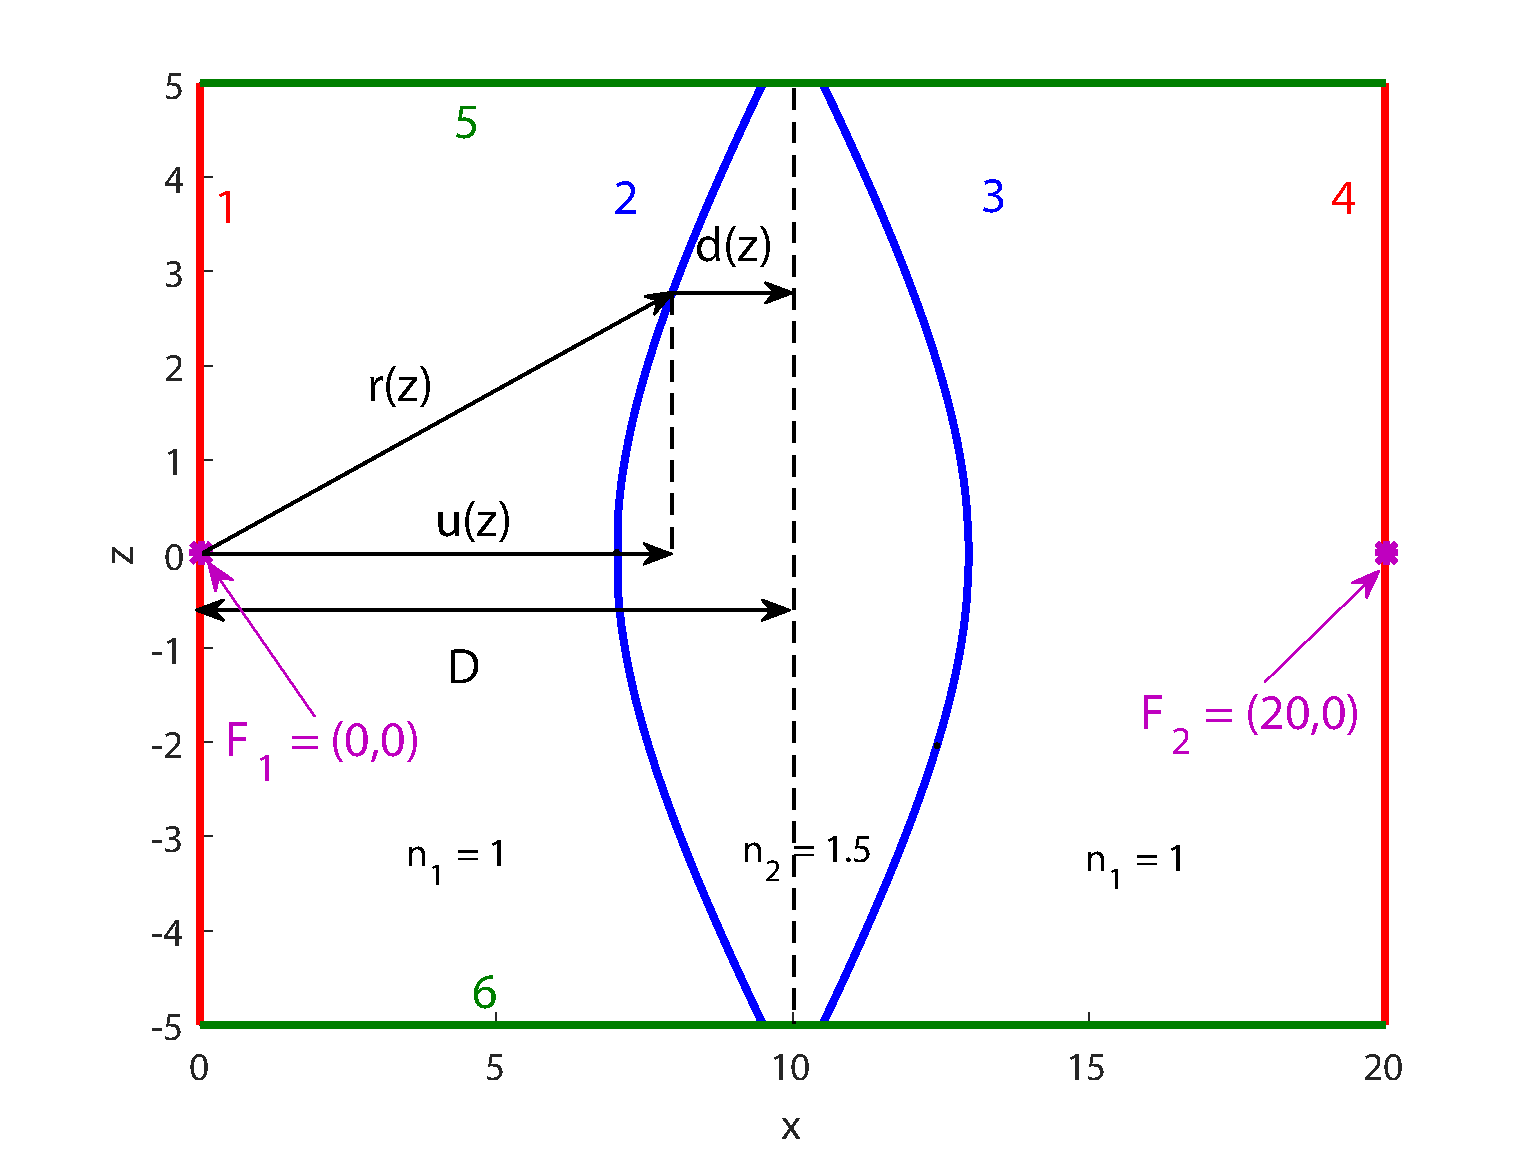
\includegraphics[width=0.7\textwidth]{lens}
  \end{center}
  \caption{\textbf{An ideal lens.} 
The source (line $1$) and the target (line $4$) are located in air ($\n = 1$), the material between lines $2$ and $3$ has index of refraction $\n=1.5$. 
Two detectors (lines $5$ and $6$) are located at the top and the bottom of the lens to detect light exiting from the system. $\point{F}_1 = (0,0)$, $\point{F}_2 = (20,0)$, $D=10$, $\variabile{h}=5$, $\variabile{d}(\variabile{h})=0.5$.}
\label{fig:lens}
 \end{figure}
It is formed by the source (line $1$), a lens formed by two optical lines (line $2$ and $3$), the target (line $4$) and two detectors (line $5$ and $6$) at the top and the bottom of the system. The source \point{S} is a vertical line segment located at $\variabile{x}=0$ with 
$\variabile{z}\in[-\variabile{h}, \variabile{h}]$, where $\variabile{h}=5$. The target \point{T} is a line segment of the same length, parallel to \point{S} and located at a distance $\variabile{x}=\variabile{a}$ from \point{S}, with $\variabile{a} = 20$. The lens is formed by two refractive lines (simple lens), and it is convex.
The lens is symmetric with respect to the axis $\variabile{x}=10$. The optical axis is the line $\variabile{z}=0$. The point $\point{F}_1 = (0,0)$ and $F_2 = (\variabile{a}, 0)$ are the focal points of line $2$ and $3$, i.e., the points where a collimated beam of light will converge after the interaction with line $2$ and $3$, respectively \cite{leutz2012nonimaging}. 
% Citation \cite{davis2007optical}
\begin{figure}[t]
  \begin{center}
  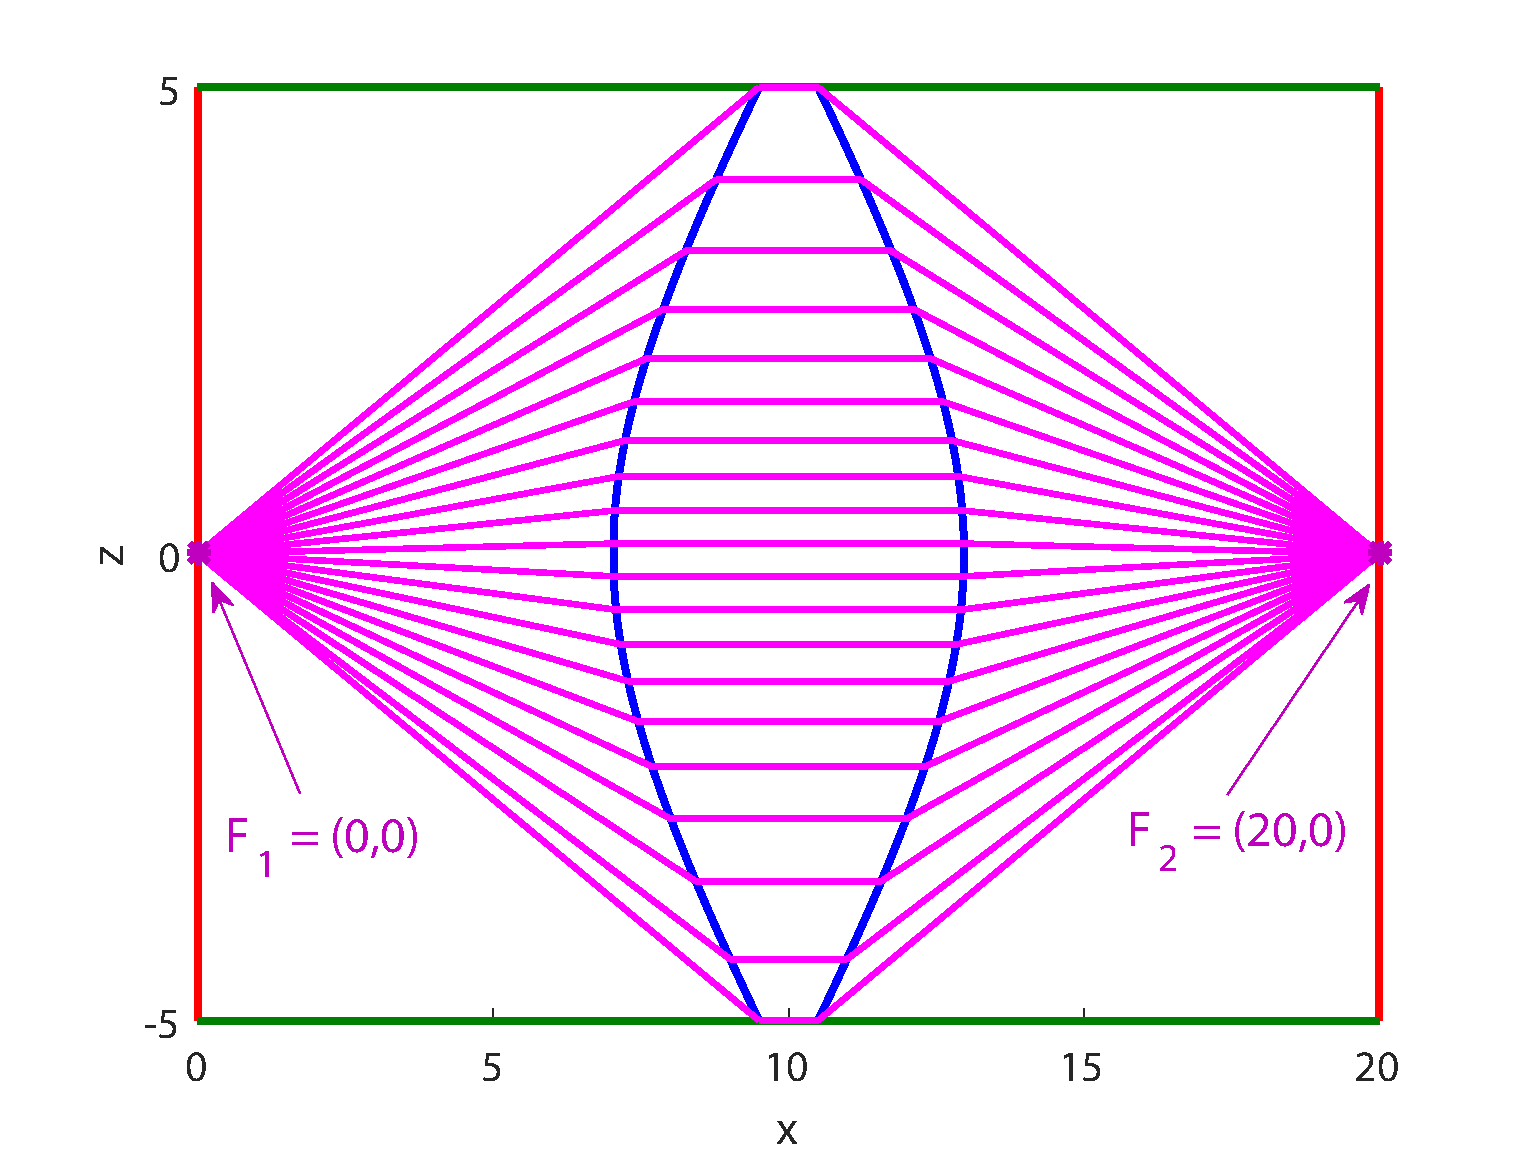
\includegraphics[width=0.7\textwidth]{lens_rays}
  \end{center}
  \caption{\textbf{An ideal lens.} 
All the rays exiting from $\point{F}_1$ arrive at $\point{F}_2$.}
\label{fig:real-lens}
 \end{figure}
\\ \indent The optical path length is defined as the product of the geometric ray path and the refractive index in which the ray travels, where the geometric ray path is the distance between two intersection points of the ray with two optical lines or the source.
The theorem of Malus-Dupin guarantees that the optical path length is constant \cite{greivenkamp2004field}. Employing this fact, we derive the equations of the lens lines. In the following we explain how the equation for the left lens (line $2$) is obtained. We indicate with $\variabile{d}(\variabile{z})$ half of the lens thickness at high $\variabile{z}$, with $\vect{r}=\vect{r}(\variabile{z})$ the parametrization of the ray emitted from $\point{F}_1$ that reaches line $2$ at height $\variabile{z}$, and $u(\variabile{z})$ the projection of $\vect{r}(\variabile{z})$ on the optical axis. 
The following relations hold:
\begin{equation}\label{eq:variables_lens}
\begin{aligned}
|\vect{r}(\variabile{z})|^{2} &= u(\variabile{z})^2+\variabile{z}^{\,2},\\
u(\variabile{z}) &= D-\variabile{d}(\variabile{z}), 
\end{aligned}
\end{equation}
The optical path length of a ray emitted from $F_1$ and arriving at a certain point of the axis $\variabile{x}=10$ is given by:
\begin{equation}\label{eq:path_length}
n_1|\vect{r}(\variabile{z})|+n_2\variabile{d}(\variabile{z})=OPL,
\end{equation}  
where $OPL>0$ is a constant obtained from the ray passing through top of the lens
\begin{equation}\label{eq:path_length2}
OPL = u(\variabile{h})+n_2\variabile{d}(\variabile{h}).
\end{equation} Substituting relations (\ref{eq:variables_lens}) and (\ref{eq:path_length}) in the previous equation,
we obtain:
\begin{equation}\label{eq:lens_equation}
a\,u(\variabile{z})^2+b\,u(\variabile{z})+c+\variabile{z}^2 = 0,
\end{equation}
for every $\variabile{z}\in[-\variabile{h}, \variabile{h}]$, where 
\begin{equation}
\begin{aligned}
a & = 1-\n_2^2, \\
b & = 2\n_2(\n_2 D-OPL), \\
c & = -(OPL-\n_2 D\,OPL)^2. \\
\end{aligned}
\end{equation}
Equation (\ref{eq:lens_equation}) leads to two real solutions, the negative one gives the expression for the left lens.
The right lens is given by a reflection with respect to the axis $\variabile{x}=0$ and a translation $(\variabile{x}, \variabile{z})\rightarrow (\variabile{x}+20, \variabile{z})$ of the expression found.
\\ \indent The lens described above has the property that every ray that hits each curved line is bent towards the optical axis. The rays passing through it connect the points $\point{F}_1 $ and $\point{F}_2$ (see Figure \ref{fig:real-lens}). Therefore, all the rays diverging from $\point{F}_1$ converge to $\point{F}_2$. In the next section we explain how to apply direct backward ray mapping to this system.
\subsection{Computation of the boundaries of the positive luminance regions}
Our goal is to show, using direct backward ray mapping, that we can detect \textit{all} the possible paths without tracing a huge number of rays. Furthermore, we are able to determine the rays that are located at the boundaries of regions corresponding to a certain physical path.
First, let us analyze the backward ray tracing process for the system in Figure \ref{fig:lens}. Every ray is traced backward from the target $\point{T}$ with an angle $\myangle_1\in[-\frac{\pi}{2}, \frac{\pi}{2}]$, i.e., with a direction coordinate $\variabile{p}_1\in[-1,1]$. Every time that a ray hits a lens, i.e., either line $2$ or $3$, the ray is split in two rays, the reflected ray and the refracted one. The reflectance $\mathcal{R}$ and the transmittance $\mathcal{T}$ are calculated. The reflected ray will continue to propagate within the system with the fraction of the power given by $\mathcal{R}$. Similarly, the transmitted ray will travel inside the system with the power given by $\mathcal{T}$. The trajectory of each ray is stopped either when it arrives at the source \point{S} or when it reaches again the target \point{T}. This leads to many different paths for a single ray with a given position and direction at the target. 
%Note that at every interaction with a Fresnel line the ray loses some energy because it is split into two more rays.
%To avoid that rays with a small power are traced through the system some ray tracing methods have been developed such that either the reflected or the refracted part of each ray is considered at every intersection with a Fresnel line. Therefore all the number of ray emitted from the source equals the number of total rays traced as no splitting is considered.  
%To detect the rays with more reflections using either MC or QMC ray tracing, more rays are needed. The number of paths possible are much more, potentially infinity paths.  
\\ \indent
Consider the target PS of the system in Figure \ref{fig:lens}. Since the source and the target are vertical lines (the $\variabile{x}$-coordinates are fixed while the $\variabile{z}$-coordinates vary), the PS coordinates at the target PS are $(\variabile{q}, \variabile{p})$, where  $\variabile{p}$ is the ray direction coordinate defined as for the previous systems and $\variabile{q}$ is the $\variabile{z}$-coordinate of the intersection point of the ray with the optical lines. To have an idea about the rays distribution at the target we calculate the target coordinates on PS of $10^5$ rays traced using MC ray tracing. MC ray tracing decides randomly which part of the ray has to be considered at every interaction with a line. This part propagates with the corresponding energy. Running MC ray tracing for the lens in Figure \ref{fig:lens} with $10^5$ rays and storing the corresponding paths, the following three paths are found:
\begin{equation}\label{eq:paths_fresnel}
\begin{aligned}
\Pi_1 & = (1,2,3,4),\\
\Pi_2 & = (1,2,3,2,3,4), \\
\Pi_3 & = (1,2,3,2,3,2,3,4).
\end{aligned}
\end{equation}
In Figure \ref{fig:target_PS_lens} we provide the target PS of the lens where we depicted rays that follow the same path with the same color. The rays in magenta are rays that follow path $\Pi_1$, the cyan rays have two reflections before reaching the target, following path $\Pi_2$, the black rays have four reflections inside the lens, these rays follow path $\Pi_3$.
\begin{figure}[t]
  \begin{center}
  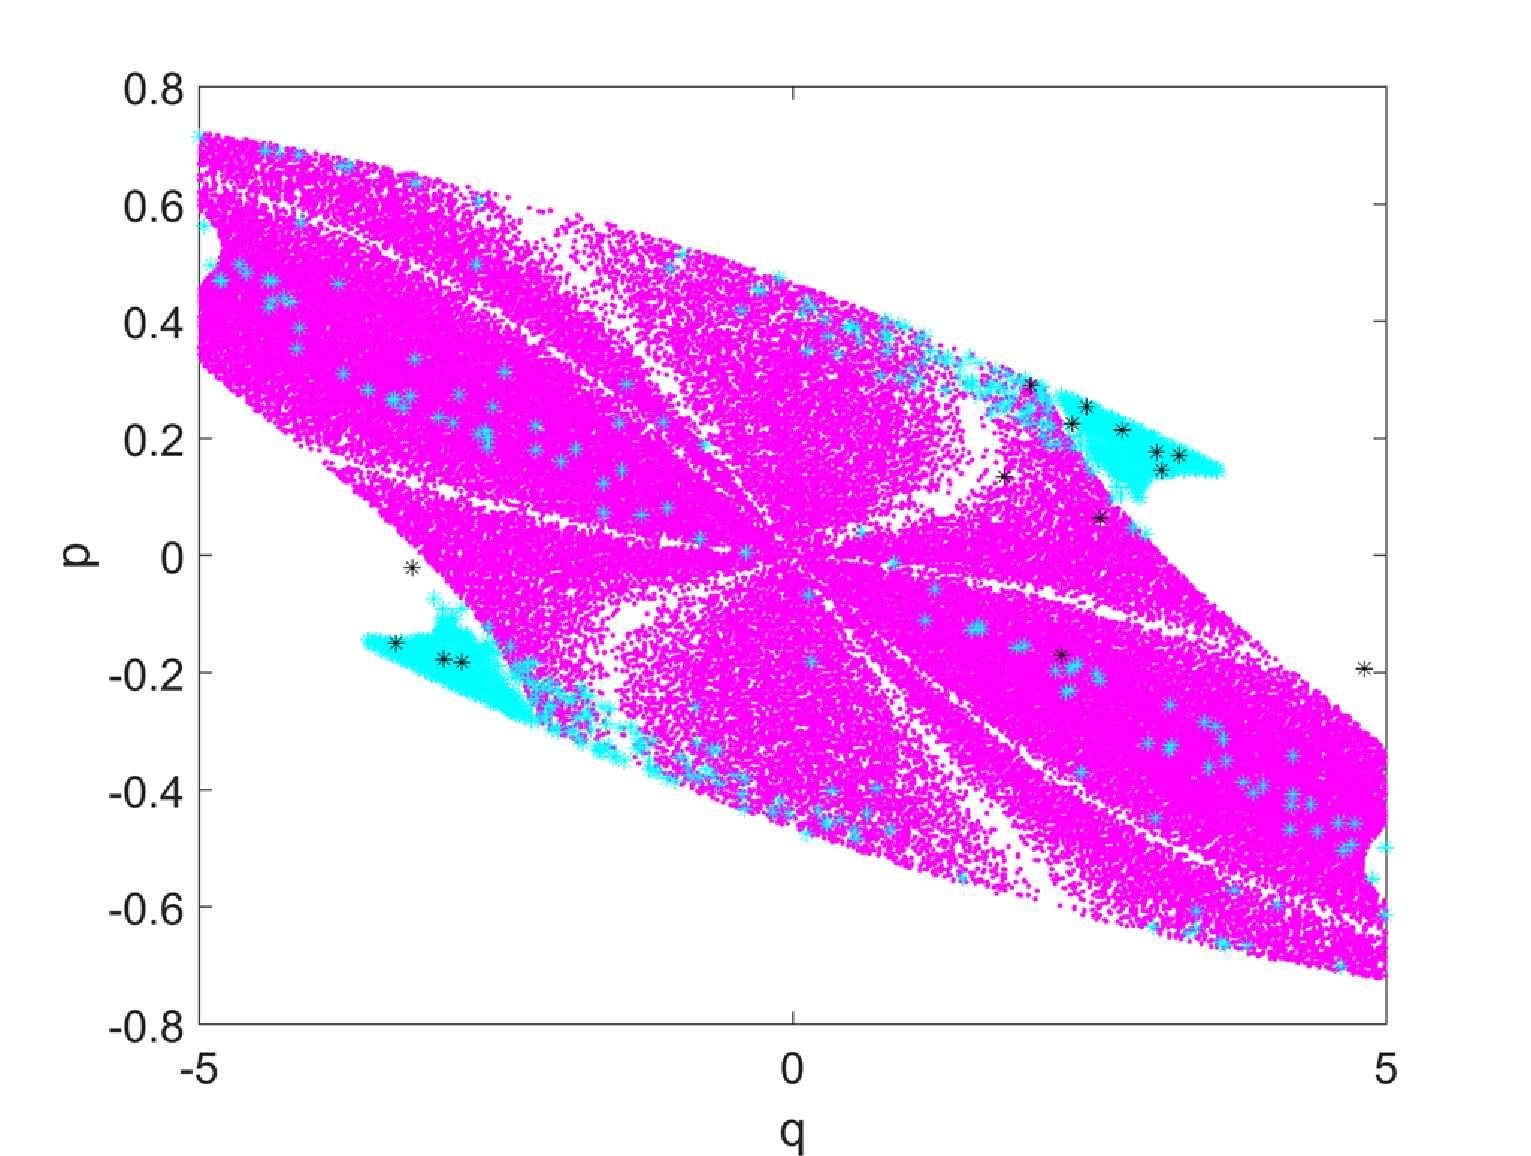
\includegraphics[width=0.7\textwidth]{target_lens}
  \end{center}
  \caption{\textbf{Target PS of the ideal lens.}
The magenta rays follow path $\Pi_1$, the cyan rays follow path $\Pi_2$ and the black rays follow path $\Pi_3$.}
\label{fig:target_PS_lens}
 \end{figure}
Note that for increasing number of reflections the corresponding rays occur less frequently in PS. 
Furthermore, there are some white parts in target PS inside the colored regions. 
This can be due to either TIR or a different choice of rays (reflected or refracted) at the intersections with Fresnel lines. In the first case, the rays will be located outside the region \set{R}{}{}$(\Pi_1)$, otherwise they can reach the interior of \set{R}{}{}$(\Pi_1)$. 
Therefore, rays that originate from two close positions at the target with close direction coordinates can follow different paths. 
Thus, given two different paths $\Pi_{\variabile{i}}$ and $\Pi_{\variabile{j}}$ with $\variabile{i}\neq\variabile{j}$, the corresponding regions \set{R}{}{}$(\Pi_{\variabile{i}})$ and \set{R}{}{}$(\Pi_{\variabile{j}})$ can overlap in target PS:
\begin{equation}
\bigcap_{\Pi}\mbox{\set{R}{}{}}(\Pi)\neq \emptyset,
\end{equation}
where the intersection is over all the possible paths. 
% Say that simply applying bisection and ray tracing is not enough
Because of this, we need to slightly modify direct backward ray mapping. \\ \indent
The key idea is to apply the bisection method of backward ray mapping for every single path $\Pi$ separately. All the possible paths from target to source can be visualized in a tree, see Figure \ref{fig:tree_fresnel}. $R$ and $T$ indicate if the reflected or the transmitted part of the ray is considered at every intersection point. Many possibilities occur, we indicate with $C$ the sequence of the choices that are made at every intersection with the lens. For example, the path $\Pi_1$ in reverse order, that is 
$\Pi_1^{\prime}=(4,3,2,1)$ corresponds to the choice $C_1= (T,T)$ from target to source (red path in Figure \ref{fig:tree_fresnel}). This means that the rays that follow path $\Pi_1$ are transmitted on both line $2$ and $3$. 
\begin{figure}[t]
  \begin{center}
  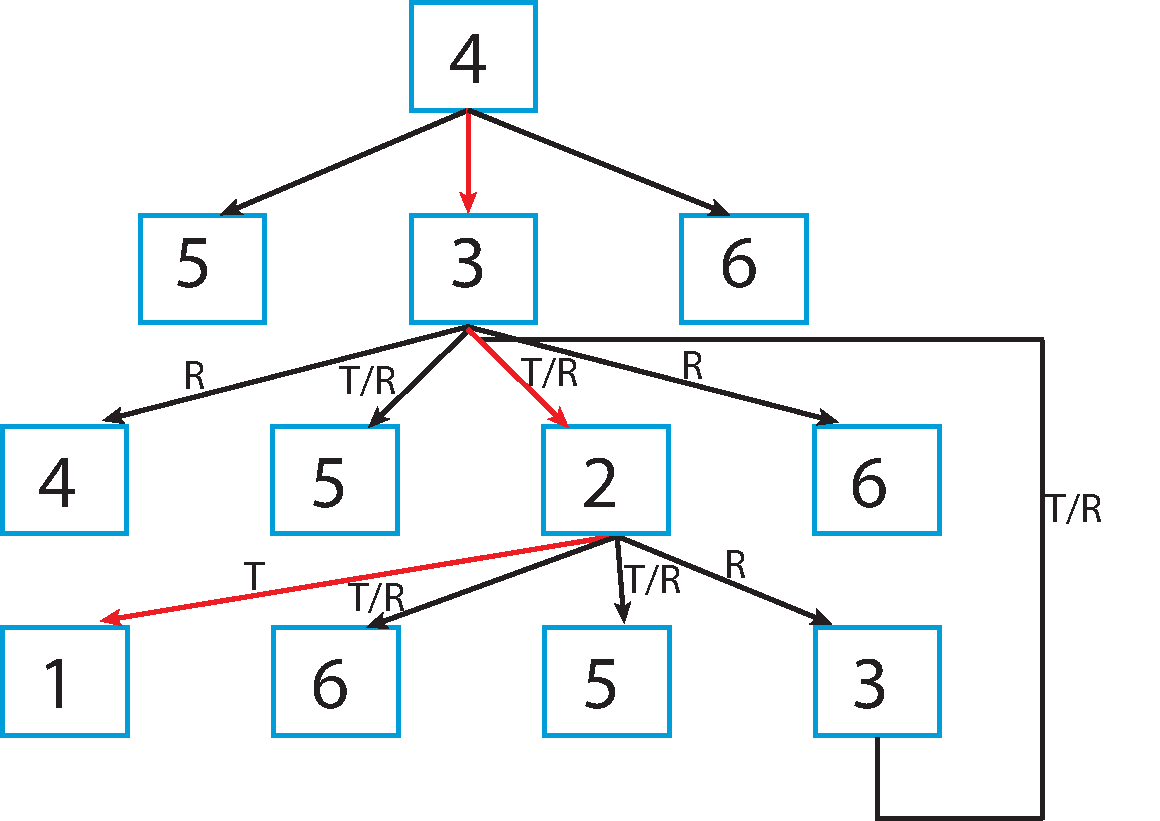
\includegraphics[width=0.7\textwidth]{tree_lens}
  \end{center}
  \caption{\textbf{Tree with all the possible paths.} Considering Fresnel reflections the rays can reflect many times between line $2$ and $3$ before reaching either the target, one of the two detectors or the source again. The inverse of path $\Pi_1 = (1,2,3,4)$ that is $\Pi_1^{\prime} = (4,3,2,1)$, is depicted in red. It corresponds to the choice $C_1= (T,T)$.}
\label{fig:tree_fresnel}
 \end{figure}
To find the intersection point of the boundary $\partial$\set{R}{}{}$(\Pi_1)$ with a line $\variabile{p} = \textrm{const}$, we start tracing back the rays with corresponding coordinates $(\variabile{q}^{\textrm{a}}, \variabile{p})$ and $(\variabile{q}^{\textrm{b}}, \variabile{p})$ located at the end points of the target PS, where $\variabile{q}^{\textrm{a}} = -\variabile{h}$ and $\variabile{q}^{\textrm{b}} = \variabile{h}$. Then the bisection method and backward ray tracing are applied as explained in the previous chapter. However, the difference with the previous method is that when the ray hits a line it is split in two rays and \textit{either} the reflected \textit{or} the refracted ray has to be selected according to the choice $C_1= (T,T)$. The corresponding energy transported by the ray is calculated at every split. This allows us to determine the coordinates of the intersection points between a line $\variabile{p}=\textrm{const}$ and the boundary $\partial$\set{R}{}{}$(\Pi_1)$. These points are denoted with $(\variabile{q}^{\variabile{i}}(\Pi_1, \variabile{p}), \variabile{p})_{\variabile{i}=1, \cdots, \variabile{r}}$ in increasing order where $\variabile{r}$ is the number of intersections point found. In case $\variabile{r}=2$ we indicate the coordinates of the two rays on the boundaries with $(\variabile{q}^{\textrm{min}}(\Pi_1, \variabile{p}), \variabile{p})$ and $(\variabile{q}^{\textrm{max}}(\Pi_1, \variabile{p}), \variabile{p})$. \\ \indent
Note that, including Fresnel reflection, the luminance at the target cannot be constant because its value depends on the Fresnel coefficients. Hence, along every direction $\variabile{p}\in[-1,1]$, we sample points in \set{R}{}{}$(\Pi_1)$ by tracing back rays with direction coordinate $\variabile{p}$ and position coordinate $\variabile{q}\in[\variabile{q}^{2i-1}(\Pi_1, \variabile{p}), \variabile{q}^{2i}(\Pi_1, \variabile{p})]$ for every $\variabile{i}=\{1, \cdots, \variabile{m}\}$ where $\variabile{m}$ is the integer part of $\variabile{r}/2$. At every interaction of each ray with a lens, either the reflected or the transmitted ray is traced further according to the choices sequence $C_1$. The energy carried by each ray is calculated. Therefore the partial luminance $L_{\Pi_1}(\variabile{q},\variabile{p})$ at the target corresponding to path $\Pi_1$ is found. 
%The interpolation between 
%$(\variabile{q}^{\textrm{min}}(\Pi_1, \variabile{p}), \variabile{p})$ and $(\variabile{q}^{\textrm{max}}(\Pi_1, \variabile{p}), \variabile{p})$ allows us to calculate the profile of $L_{\Pi_1}(\variabile{q},\variabile{p})$ for every $\variabile{q}\in[\variabile{q}^{\textrm{min}}, \variabile{q}^{\textrm{max}}]$ and $\variabile{p}=\textrm{const}$.
% as it depends on the Fresnel coefficients which are related to the angle of the incident ray at every Fresnel line and to the index of refraction in which the ray travels (see equations (\ref{eq:fresnel_pands2})). Therefore and interpolation between the coordinates of the rays on the boundaries gives the value of the luminance $L_{\Pi_1}(\variabile{q}, \variabile{p})$ along direction $\variabile{p}= \textrm{const}$ related to path $\Pi_1$.
Repeating the procedure for all the possible directions $\variabile{p}\in[-1,1]$, the profile of the partial luminance $L_{\Pi_1}$ at the target given by all the rays that follow path $\Pi_1$ is computed for every $(\variabile{q}, \variabile{p})\in$\set{T}{}{}. 
\\ \indent Next, another path $\Pi$ and the corresponding sequence of choices $C$ are considered. We remark that every path is associated to a unique choice but the reverse is not always true. For example, the path $\Pi_2 = (1,2,3,2,3,4)$ considered in reverse order from \point{T} to \point{S}, i.e., $\Pi_2^{\prime} = (4,3,2,3,2,1)$ can only be associated to sequence $C_2 = (T,R,R,T)$. However, this sequence also corresponds with the two inverse paths $\Pi_5^{\prime}= (4,3,2,3,2,5)$ and $\Pi_6^{\prime}= (4,3,2,3,2,6)$. The last two paths $\Pi_5^{\prime}$ and $\Pi_6^{\prime}$ are not realistic paths from target to source, therefore they are discarded for the intensity calculation. Given a sequence $C$, many paths are possible but only one is the physical path. In the flowchart in Figure \ref{fig:flowchart_fresnel}, we show all the steps needed to calculate the partial luminance $L_{\Pi_1}(\variabile{q}, \variabile{p})$  along a given direction $\variabile{p}$ and related to path $\Pi_1 = (1,2,3,4)$ which corresponds to the sequence of choices $C= (T,T)$. The procedure to determine the other paths is similar.
\begin{figure}[t]
  \begin{center}
  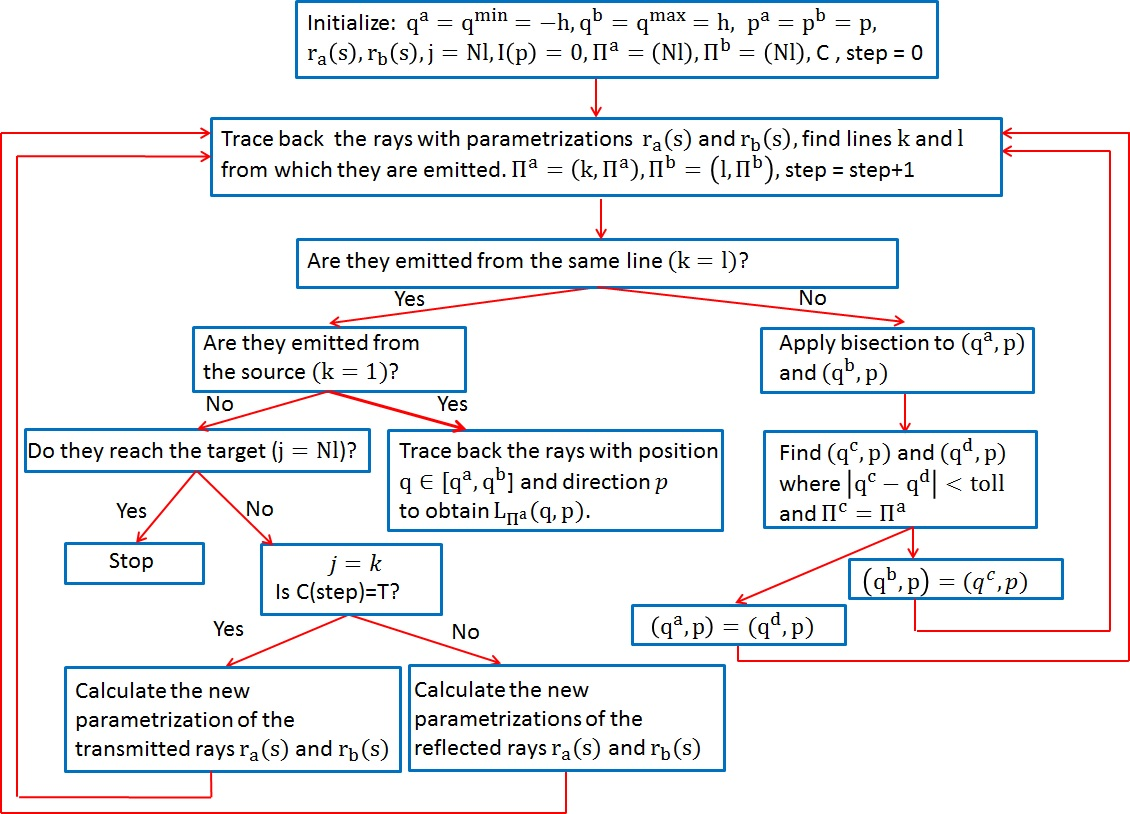
\includegraphics[width=\textwidth]{flowchart_fresnel3}
  \end{center}
  \caption{\textbf{Main steps of backward ray mapping extended to systems with Fresnel reflection.}}
\label{fig:flowchart_fresnel}
 \end{figure}
%Considering \textit{all} the possible sequences of choices, \textit{all} the physical paths are determined. The corresponding partial luminance $L_{\Pi}(\variabile{q}, \variabile{p})$ along every direction $\variabile{p}\in [-1,1]$ and for every position coordinate $\variabile{q}\in[\variabile{q}^{\textrm{min}}(\Pi, \variabile{p}), \variabile{q}^{\textrm{max}}(\Pi, \variabile{p})]$ is calculated for every path $\Pi$. 
\\ \indent Finally, the total luminance $L(\variabile{q}, \variabile{p})$ is given by:
\begin{equation}\label{eq:luminance_fresnel}
L(\variabile{q}, \variabile{p}) = \sum_{\Pi}L_{\Pi}(\variabile{q}, \variabile{p}),
\end{equation} 
where the summation is over all the possible paths. 
From an integration of $L(\variabile{q}, \variabile{p})$ the intensity at the target is given by:
\begin{equation}\label{eq:intensity_fresnel}
I(\variabile{p}) = \int_{\mbox{\set{Q}{}{}}}L(\variabile{q}, \variabile{p})\textrm{d}\variabile{q}.
\end{equation}
In the next section numerical results are shown.
\section{Numerical results}
In this section the numerical results for the lens are presented. We detect the boundaries of the regions formed by the rays that follow the same path. To this purpose we decide a priori the sequence of choices that has to be made at every intersection. This sequence determines whether the reflected or the transmitted part of the incident ray has to be considered when the rays traced back hit a line.\\ \indent
We start with the sequence of choices $C_1 = (T,T)$ which corresponds to the physical path $\Pi_1=(1,2,3,4)$.
Indeed, every ray traced back hits the right curved line (line $3$) and is split in two rays, at this point the reflectance $\mathcal{R}$ and transmittance $\mathcal{T}$ are calculated and, according to the first component of $C_1$, the transmitted ray is considered and traced back further with the corresponding power $\mathcal{T}$. This ray continues to propagate through the system until it hits either the detectors (line $5$ and $6$) or the curved line $2$.
In case it hits the detectors the procedure is stopped, otherwise the ray is split again into two more rays. Now, according to the second component of $C_1$, the transmitted ray is considered and it continues its trajectory reaching either one of the detectors or the source (line $1$). For example, in Figure \ref{fig:ray_path1} we draw in magenta a ray that follows the inverse path $\Pi_1^{\prime} = (4,3,2,1)$. It is traced back from the target and has target PS coordinates $(\variabile{q}, \variabile{p})=(0, -0.4)$. It arrives at the source with $55\%$ of the initial power.\\ \indent 
Using direct backward ray mapping and taking into account the choice $C_1$, the boundary $\partial$\set{R}{}{}$(\Pi_1)$ is found which is the blue line in Figure \ref{fig:boundary_path1}. To verify whether this boundary is correct we trace around $10^4$ rays using MC ray tracing imposing that at every interaction of the ray with lines $2$ and $3$ always the transmitted part is considered. These rays are displayed in magenta in Figure \ref{fig:boundary_path1}. The picture shows that all the rays traced are inside the boundary $\partial$\set{R}{}{}$(\Pi_1)$. So we conclude that the boundary is calculated correctly.
\begin{figure}[t]
\centering
\begin{subfigure}[t]{.45\textwidth}
  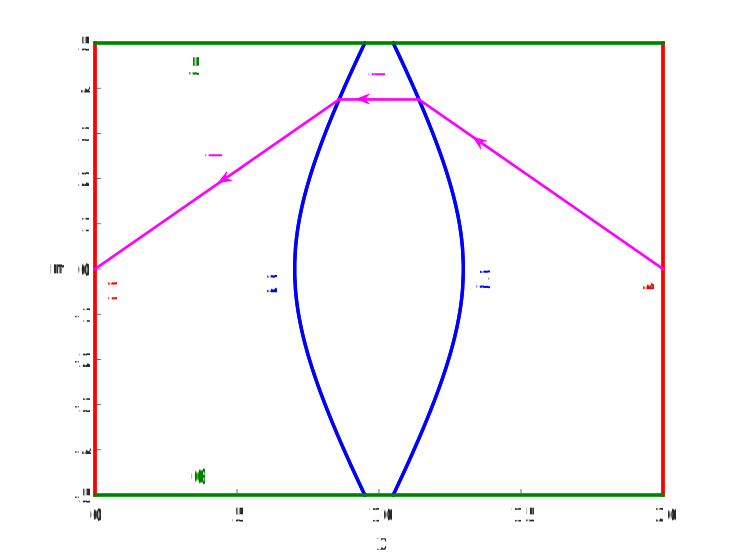
\includegraphics[width=\textwidth]{lens_path1}
 \caption{\textbf{Ray traced back from target to source}. The ray follows inverse path $\Pi_1^{\prime} = (4,3,2,1)$ corresponding to the choice $C_1=(T,T)$ from target to source. The percentage of power of the ray at the source is approximately $55\%$ of the initial power.}
  \label{fig:ray_path1}
\end{subfigure}%
\hfill
\begin{subfigure}[t]{.45\textwidth}
  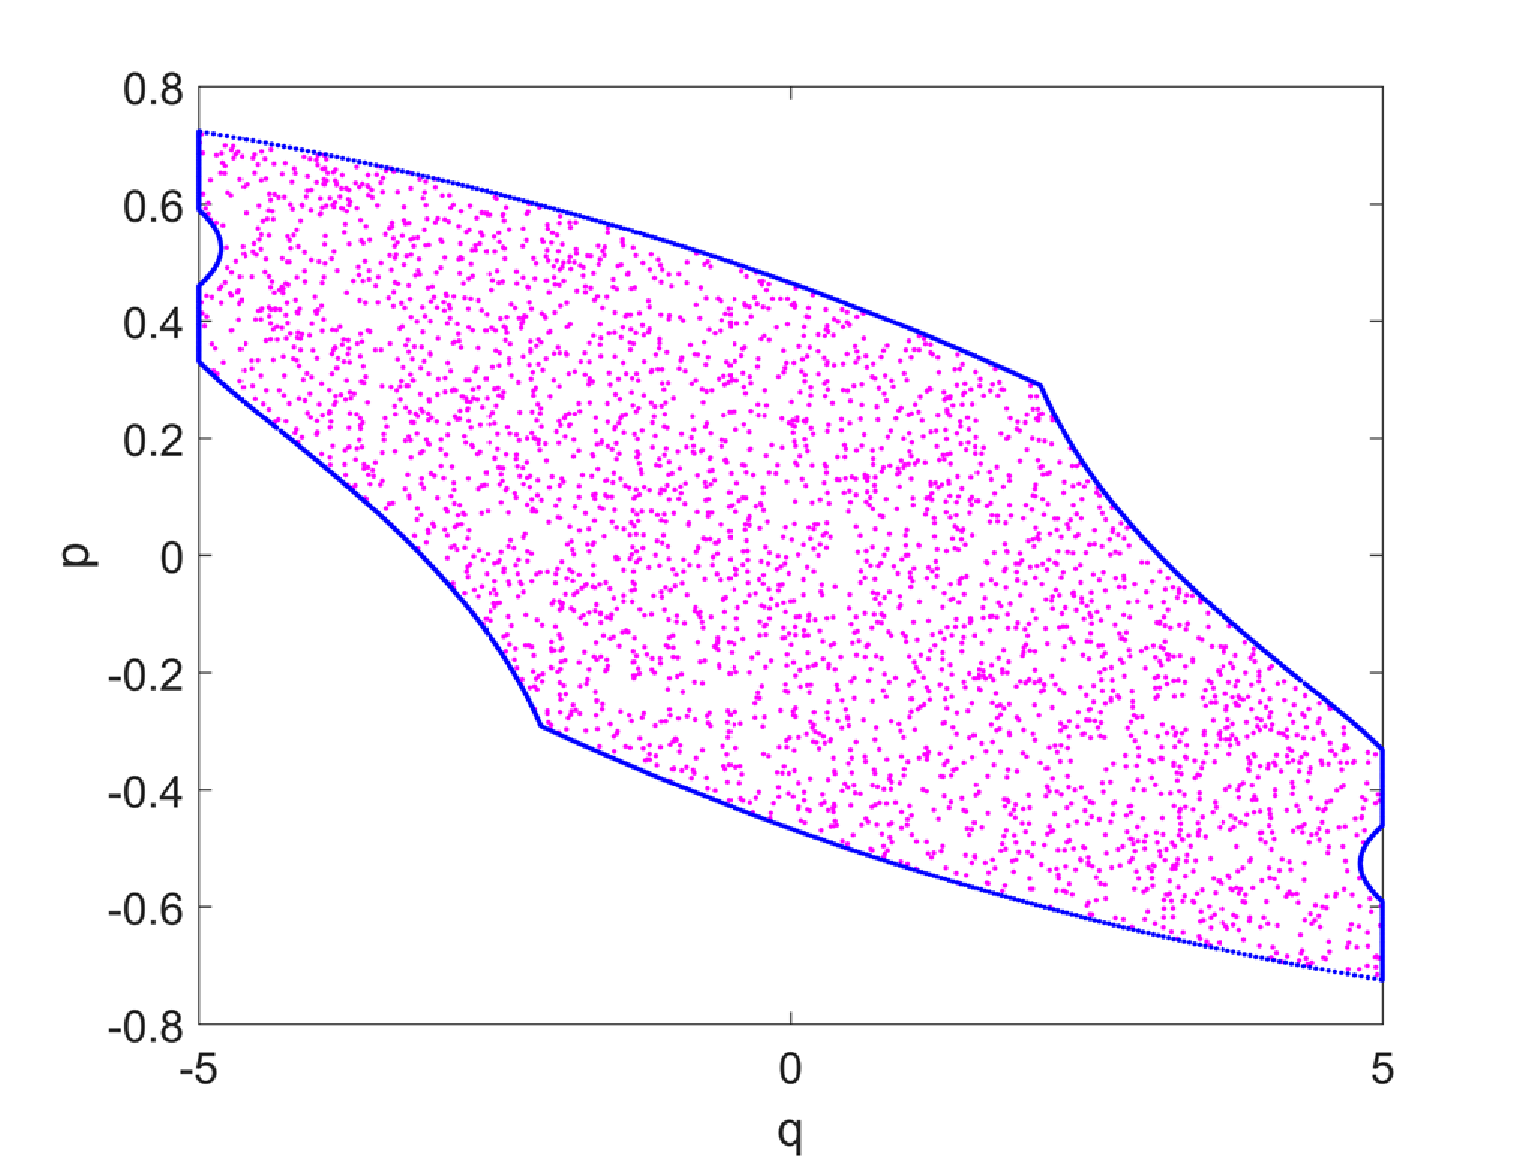
\includegraphics[width=\textwidth]{path_lens1}
  \caption{\textbf{Boundary $\partial$\set{R}{}{}$(\Pi_1)$.} The boundary is depicted with the blue line, the magenta rays are traced using MC ray tracing and considering always the transmitted ray.} %
  \label{fig:boundary_path1}
\end{subfigure} %
\caption{\textbf{Computation of the boundary $\partial$\set{R}{}{}$(\Pi_1)$.}}
\end{figure}
\\ \indent To detect the other paths we need to consider all possible sequences. We continue with $C_2 = (T, R, R, T)$. This means that if a ray traced back from the target hits line $3$, the transmitted part is considered according to the first component of $C_2$. Next, it is traced back further with its corresponding power given by $\mathcal{T}$. If the transmitted ray does not hit one of the detectors, it hits line $2$ where it is split again. Now the reflected part of the ray is considered according to the second component of $C_2$. The power of the reflected ray is given by the product $\mathcal{R}\mathcal{T}$. Note that, in the case of unpolarized light, the product $\mathcal{R}\mathcal{T}$ depends on the angle of incidence of the ray (see Equations (\ref{Fresnel_pands}) and (\ref{eq:RandTin2D})). The ray continues to propagates inside the system, if it hits line $3$ it is reflected according to the third component of $C_2$ and, in case it hits line $2$ next, it is finally transmitted according to the last component of $C_2$. If the ray finally reaches the source, it has followed the inverse path $\Pi_2^{\prime} = (4,3,2,3,2,1)$. 
In Figure \ref{fig:ray_path2} we show in cyan a ray traced back from target to source that follows path $\Pi_2$. The ray with target PS coordinates $(\variabile{q}, \variabile{p})=(0,-0.37)$ is traced back and after two reflections inside the lens it arrives at the source with $7.2\%$ of the initial energy. Direct backward ray mapping combined with sequence $C_2$ provides the boundary of the region $\partial$\set{R}{}{}$(\Pi_2)$ which is depicted in blue in Figure \ref{fig:boundary_path2}. To properly detect the boundary we divided the target PS into $\textrm{Ni}=10$ bins as explained in Section \ref{sec:TIR}. Like for the boundary $\partial$\set{R}{}{}$(\Pi_1)$, to prove that the method computes the boundary correctly we traced $10^4$ rays using MC ray tracing in combination with sequence $C_2$. These rays are shown in cyan in Figure \ref{fig:boundary_path2}. 
\begin{figure}[t]
\centering
\begin{subfigure}[t]{.45\textwidth}
  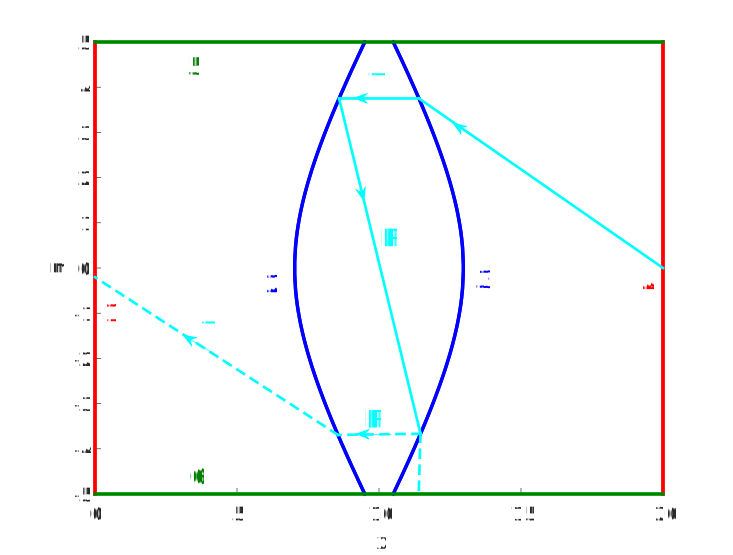
\includegraphics[width=\textwidth]{lens_path2}
 \caption{\textbf{Ray traced back from target to source}. The ray follows inverse path $\Pi_2^{\prime} = (4,3,2,3,2,1)$ corresponding to the choice $C_2=(T,R,R,T)$ from target to source. The percentage of power of the ray at the source is $7.2\%$ of the initial energy.}
  \label{fig:ray_path2}
\end{subfigure}%
\hfill
\begin{subfigure}[t]{.45\textwidth}
  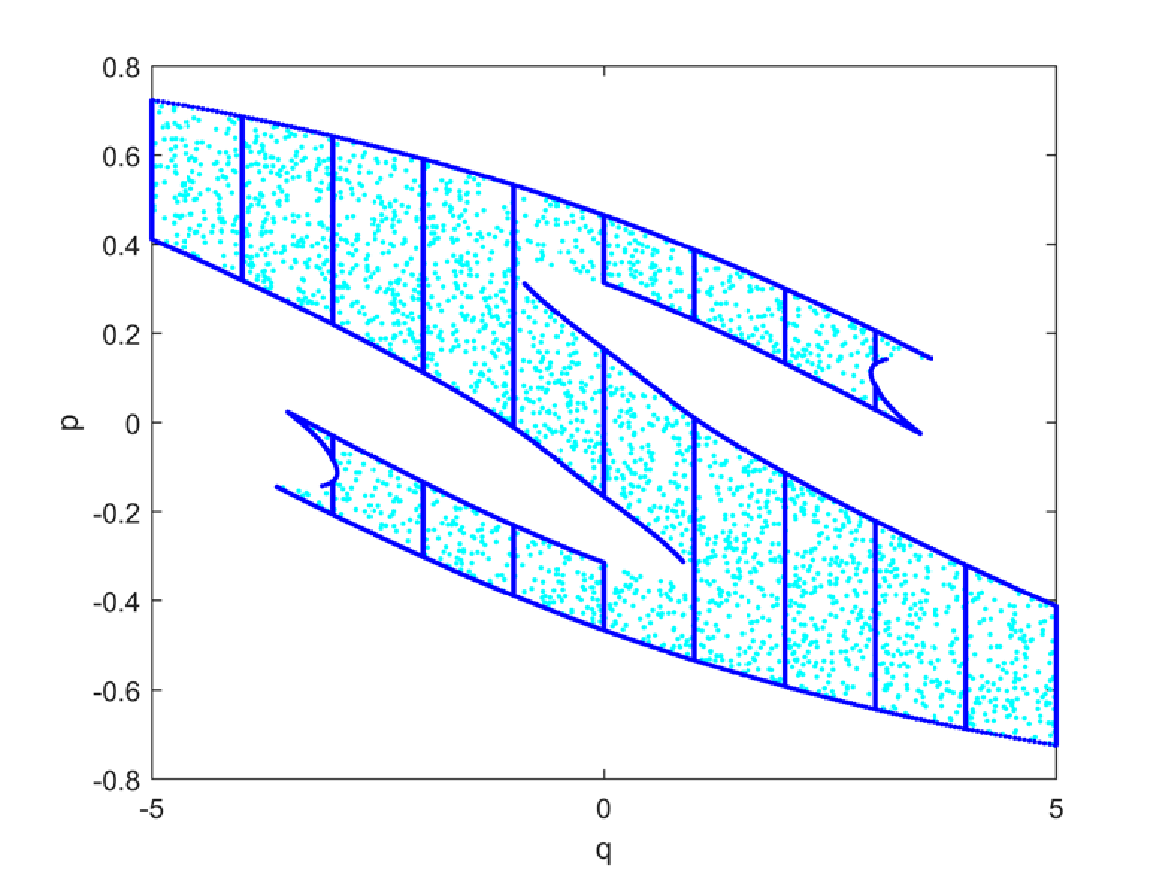
\includegraphics[width=\textwidth]{path_lens2}
  \caption{\textbf{Boundary $\partial$\set{R}{}{}$(\Pi_2)$.} The boundary is depicted with the blue line, the cyan rays are traced using MC ray tracing with $10^4$ and considering two reflections between the lenses.} %
  \label{fig:boundary_path2}
\end{subfigure} %
\caption{\textbf{Computation of the boundary $\partial$\set{R}{}{}$(\Pi_2)$.}}
\end{figure}
\\ \indent Since more than two reflections can occur between line $2$ and $3$, the procedure continues considering the sequence $C_3 = (T,R,R,R,R,T)$ leading to four reflections between line $2$ and $3$. Every ray traced back from the target is first transmitted, then reflected between $2$ and $3$ four times and finally transmitted again. If the ray hits the source then it has followed the inverse path $\Pi_{3}^{\prime} = (4,3,2,3,2,3,2,1)$ corresponding to sequence $C_3$. An example of a ray that follows path $\Pi_3$ is depicted in black in Figure \ref{fig:ray_path3}. The ray is traced back from the target with target PS coordinates $(\variabile{q}, \variabile{p})=(0,-0.39)$. It arrives at the source with a power equal to $0.0073\%$ of the initial energy. The backward ray mapping with the sequence $C_3$ gives the boundary $\partial$\set{R}{}{}$(\Pi_3)$ depicted in blue in Figure \ref{fig:boundary_path3}. This boundary is obtained dividing the target PS into $\textrm{Ni}=10$ bins and applying the backward ray mapping to each bin. The black dots correspond to the rays in target PS obtained using MC ray tracing in combination with sequence $C_3$ with $10^4$ rays.
\begin{figure}[t]
\centering
\begin{subfigure}[t]{.45\textwidth}
  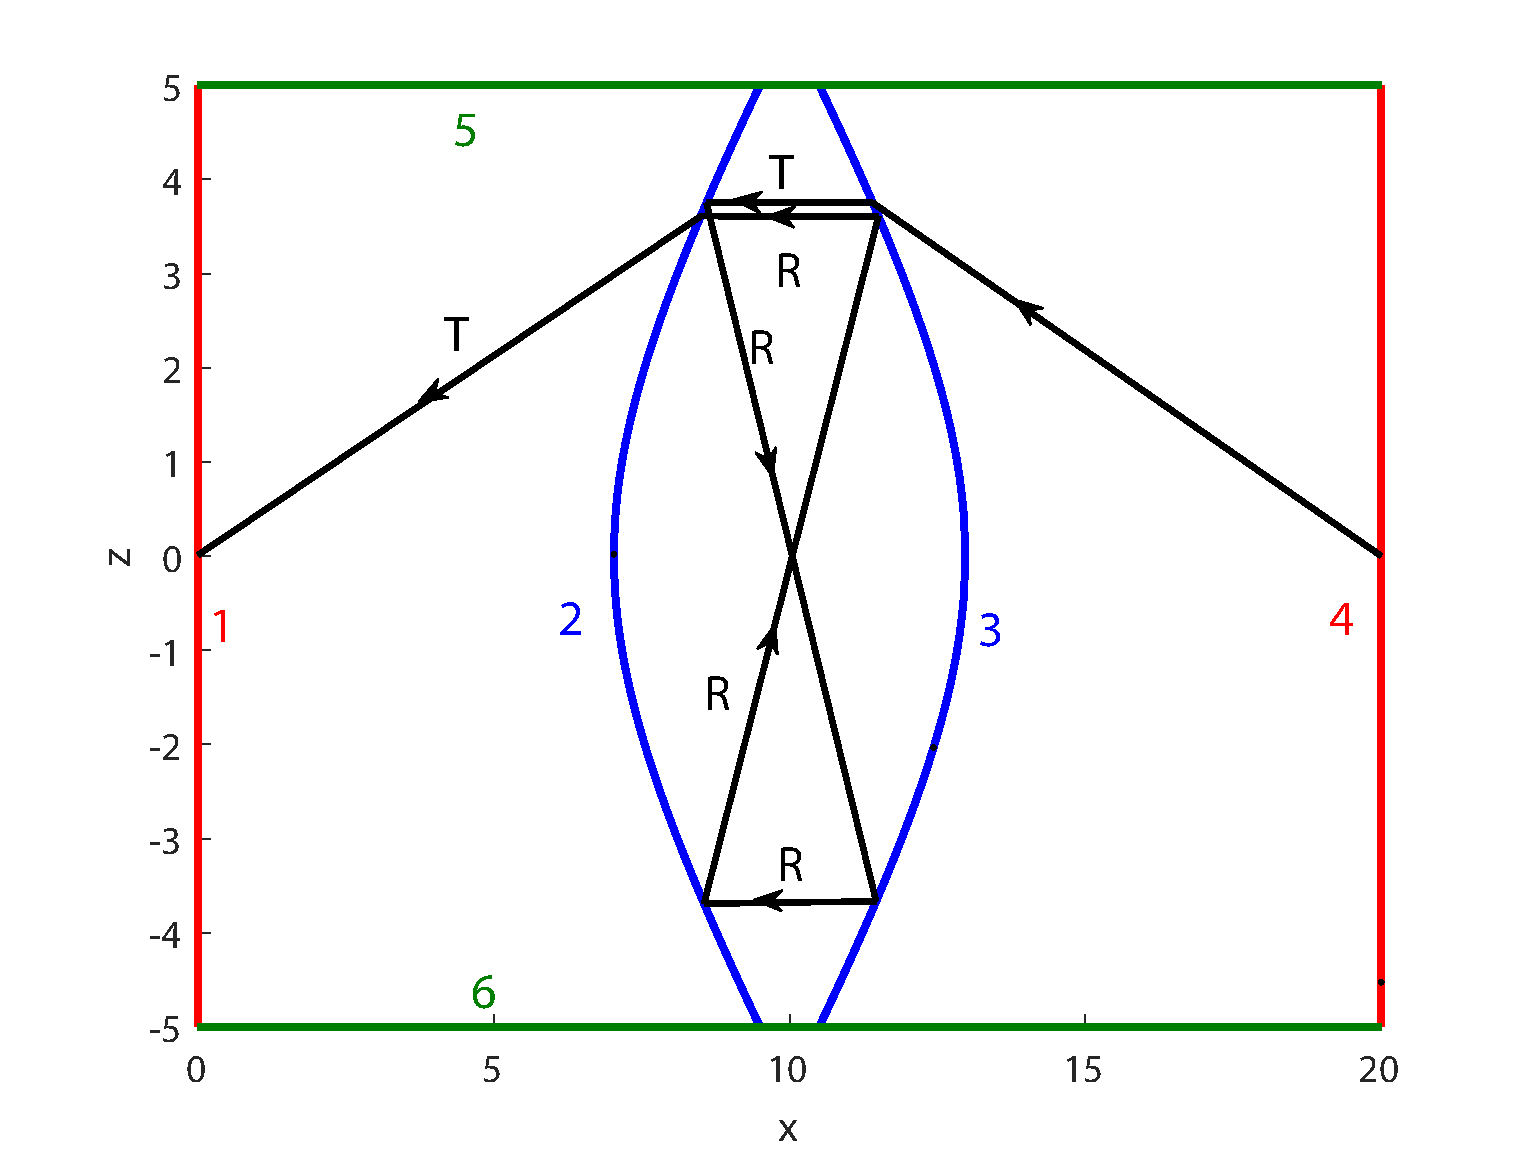
\includegraphics[width=\textwidth]{lens_path3}
 \caption{\textbf{Ray traced back from target to source}. The ray follows inverse path $\Pi_3 = (4,3,2,1,2,3,2,1)$ corresponding to the sequence of choices $C_3=(T,R,R,R,R,T)$ from target to source. The percentage of power of the ray at the source is $0.0073\%$ of the initial energy.}
  \label{fig:ray_path3}
\end{subfigure}%
\hfill
\begin{subfigure}[t]{.45\textwidth}
  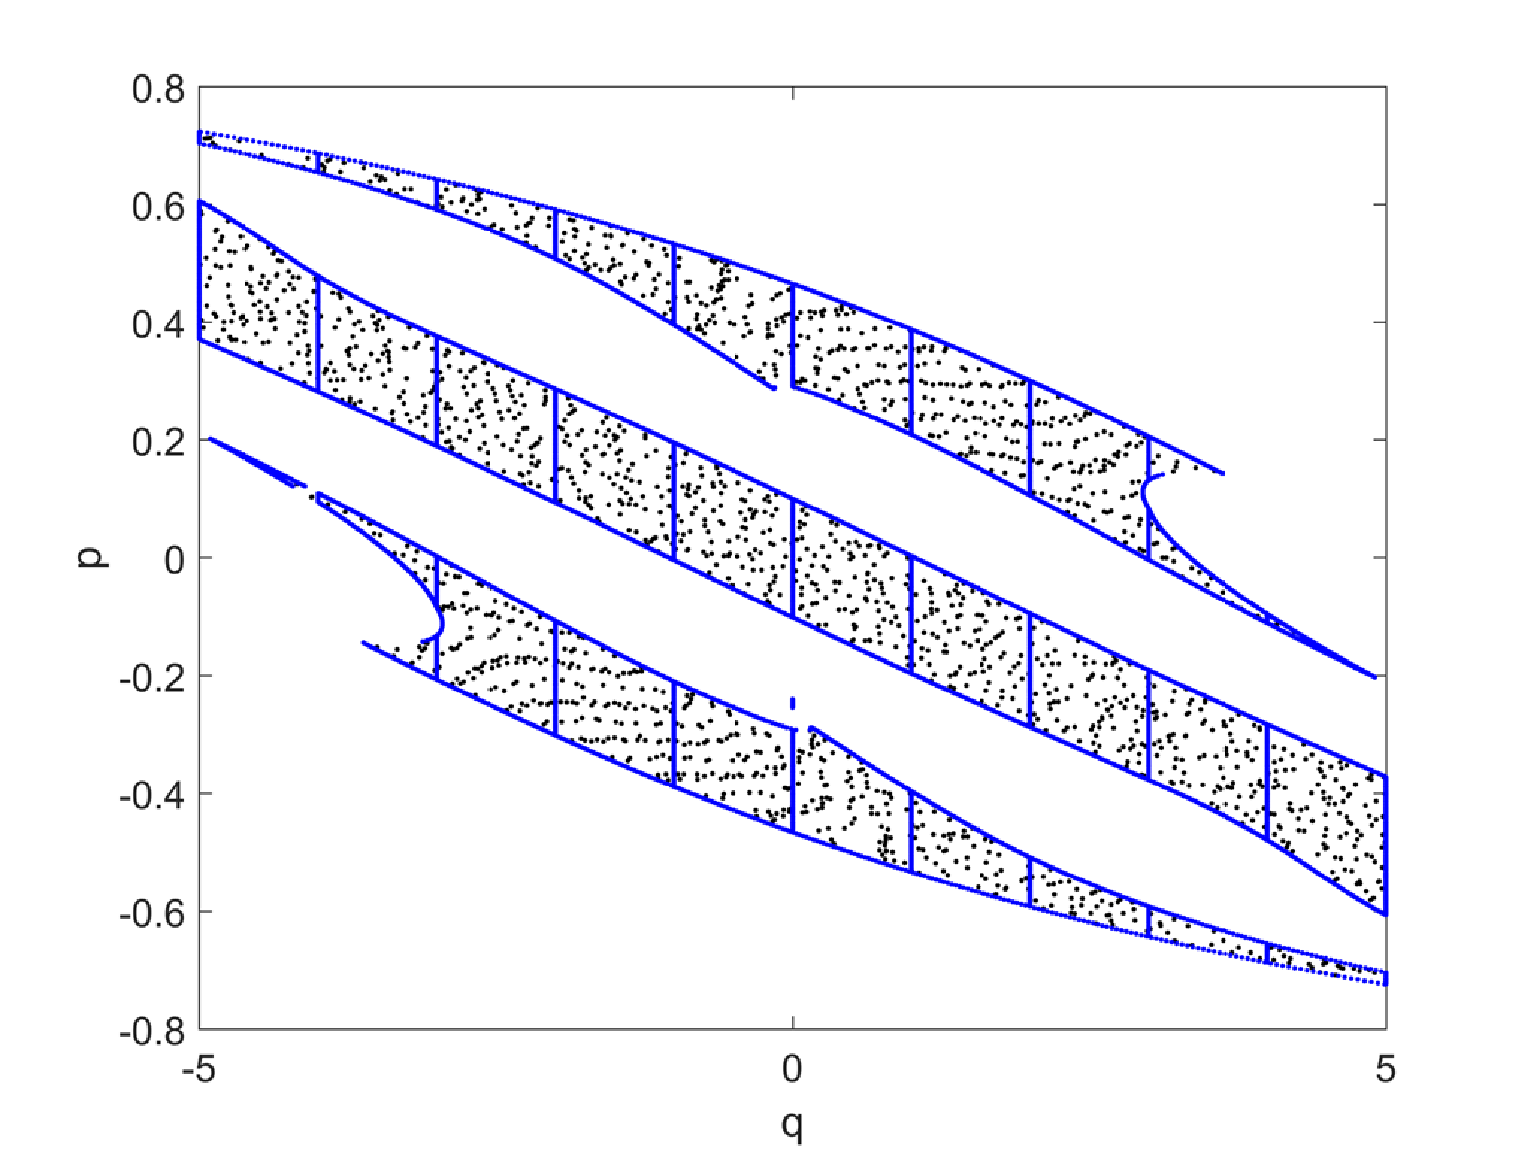
\includegraphics[width=\textwidth]{path3_fresnel}
  \caption{\textbf{Boundary $\partial$\set{R}{}{}$(\Pi_3)$.} The boundary is depicted with the blue line, the black rays are traced using MC ray tracing with $10^4$ and considering four reflections between the lenses.} %
  \label{fig:boundary_path3}
\end{subfigure} %
\caption{\textbf{Computation of the boundary $\partial$\set{R}{}{}$(\Pi_3)$.}}
\end{figure}
\\ \indent 
Direct backward ray mapping is able to detect \textit{all} the boundaries of \textit{all} regions of positive luminance in target PS. Since rays with multiple reflections hardly contribute to the total power, we discard rays with more than four reflections. The procedure can be stopped according to the desired accuracy. The more reflections are considered, the better the accuracy. \\ \indent
Note that the luminance at the target cannot be constant because every ray carries a certain amount of energy that depends on the Fresnel coefficients. Because of this, a sampling in the interior of the boundaries is needed to compute the profile of the luminance at the target. 
%In Figure \ref{fig:interpolation1}
Next we explain the procedure to compute the luminance with an example related to path $\Pi_1$ along direction $\variabile{p}=0$. A sample of rays with corresponding coordinates $(\variabile{q}, \variabile{p})$ where $\variabile{q}\in[\variabile{q}^{\textrm{min}}(\Pi_1,\variabile{p}), \variabile{q}^{\textrm{max}}(\Pi_1,\variabile{p})]$ and $\variabile{p}=0$ need to be traced from the target to the source using the backward ray tracing and taking into account sequence $C_1$. The luminance $L_{\Pi_1}(\variabile{q}, \variabile{p})$ is calculated for every $\variabile{q}\in[\variabile{q}^{\textrm{min}}(\Pi_1,\variabile{p}), \variabile{q}^{\textrm{max}}(\Pi_1,\variabile{p})]$ and $\variabile{p}=0$. 
%Its profile is depicted in Figure \ref{fig:luminance_fresnel}.
%\begin{figure}[t]
%\centering
%\begin{subfigure}{.45\textwidth}
%  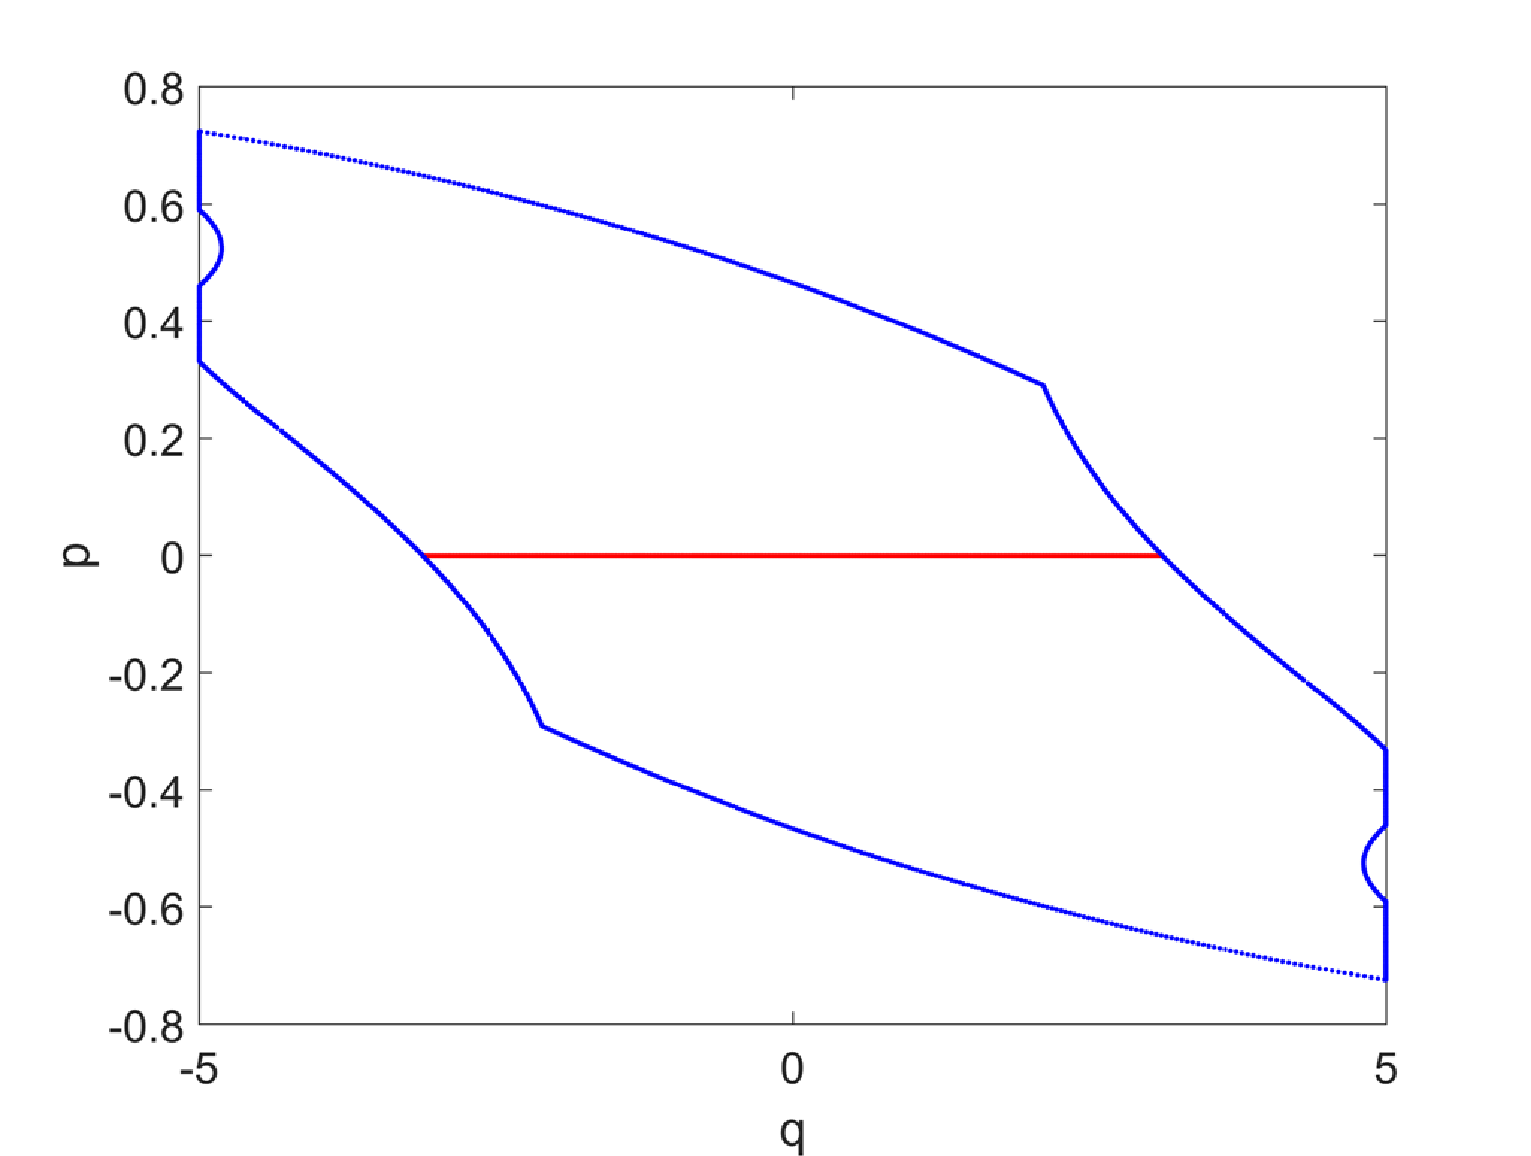
\includegraphics[width=\textwidth]{interpolation1}
% \caption{Sample of rays in the interior of $\partial$\set{R}{}{}$(\Pi_1)$ along direction $\variabile{p}=0$.}
%  \label{fig:interpolation1}
%\end{subfigure}%
%\hfill
%\begin{subfigure}{.45\textwidth}
%  \includegraphics[width=\textwidth]{luminance}
%  \caption{Luminance $L_{\Pi_1}(\variabile{q}, 0)$ related to path $\Pi_1$ along direction $\variabile{p}=0$ and with $\variabile{q}\in[\variabile{q}^{\textrm{min}}(\Pi_1, \variabile{p}), \variabile{q}^{\textrm{max}}(\Pi_1, \variabile{p})]$.} %
%  \label{fig:luminance_fresnel}
%\end{subfigure} %
%\caption{\textbf{Determination of the partial luminance.} $L_{\Pi_1}(\variabile{q}, 0)$ is related to path $\Pi_1$ along direction $\variabile{p}=0$.} 
%\end{figure}
\\\indent 
Repeating the procedure explained above along all possible directions $\variabile{p}\in[-1,1]$, the partial luminance $L_{\Pi_1}(\variabile{q}, \variabile{p})$ is found for every $\variabile{q}\in[\variabile{q}^{\textrm{min}}(\Pi_1,\variabile{p}), \variabile{q}^{\textrm{max}}(\Pi_1,\variabile{p})]$ and $\variabile{p}\in[-1,1]$. The same procedure is applied to all the paths considered and the luminance corresponding to each path is calculated. The total luminance $L(\variabile{q}, \variabile{p})$ is given by the sum in (\ref{eq:luminance_fresnel}). Finally, the intensity is computed using (\ref{eq:intensity_fresnel}). \\ \indent
We do not show here the numerical results of the total luminance and intensity because the work is still in progress. Our expectation is that direct backward ray mapping is suitable also for systems with Fresnel reflection. Indeed, the preliminary results show that the boundaries of the regions with positive luminance are calculated correctly. Once the boundaries are found also the luminance and the intensity can be computed applying an interpolation between the rays at the boundaries along every possible direction. Furthermore we expect that the method is much more accurate and faster than both MC and QMC ray tracing. This because we can analyze every single path independently.  
\section{Conclusion and outlook}
In this chapter we extended direct backward ray mapping to optical systems where Fresnel reflections play a role. We observed that a ray emitted from the source follows many different paths as it is split into two rays every time that it hits a line. Thus, a unique point at source PS will correspond to several points at target PS. This results in an overlap of the regions with positive luminance in target PS. The purpose of the method is to detect the boundaries of \textit{all} these regions. This can be done fixing a priori which part of the ray has to be considered at every intersection of the ray with a Fresnel line. \\\indent Direct backward ray mapping is extended in this chapter such that only one boundary is computed at each run. The procedure is run as many times as the number of sequences of choices we want to consider. We presented preliminary numerical results for a system formed by the source, the target and a lens formed by two curved lines. We have shown that the method is able to determine the boundaries of all the regions with positive luminance correctly. We noticed that, including Fresnel reflections, the luminance cannot be constant. An interpolation between the rays on the boundaries is needed to obtain the luminance profile. 
%We provided an example of such interpolation for a given path and along a certain direction.
Furthermore, we explained the theory for the luminance and the intensity computation. \\ \indent
Future work might regard the calculation of the luminance and the intensity and a comparison with both MC and QMC ray tracing. Numerical results on the intensity computation should be provided.





